%Die Angabe des schlauen Spruchs auf diesem Wege funtioniert nur,
%wenn keine Änderung des Kapitels mittels den in preambel/chapterheads.tex
%vorgeschlagenen Möglichkeiten durchgeführt wurde.
\chapter{Problem Definition and Feature Selection}
\label{chap:chapter4}
%\vspace{-3cm}
%\vspace{2cm}
There are number of methods to separate permanent faults from non-recurring faults as explained in section~\ref{sec:secfc}. However available techniques do not separate faults as permanent, transient and intermittent. This is of particular importance from point of view of reducing yield loss, by including chips which showed only transient faults. Also, if faults can be categorized into these categories, then it gives an additional information to designer about the underlying fault mechanism, so that additional optimization of yield can be achieved. 

The classification approaches explained in section~\ref{sec:secfc} are mostly rule or heuristic based (e.g. threshold value in $\alpha$-counting techniques) and these heuristics or rules will change every time technology is node to lower nodes, hence these rules become obsolete over time. An elaborate analysis is required to update these rules for every product and technology.

Generally speaking, when an intermittent fault occurs in a system, its activation rate is higher than the transient fault rate \cite{Bondavalli2000}. However, as systems are moving to lower technology nodes, transient faults are also on the rise, as explained in section~\ref{sec:secft}. Hence with traditional techniques, it becomes difficult to separate transients from intermittents using $\alpha$-count, as the fault rates for these two types of faults become close to each other.

This calls for an automated and adaptive approach which is independent on product and technology and that can classify faults as intermittent, transient and permanent. 

\section{Machine learning approach for fault classification}

Machine learning has been used in wide variety of classification applications with reasonable accuracy \cite{Pang2002,Nguyen2008,Sebastiani2002, Kotsiantis2007}. As explained in chapter~\ref{chap:chapter3}, machine learning is used when it is not practical to arrive at rules by looking at the data. Machine learning algorithms can be implemented as \enquote{black-box} approach for classification and all user needs to do is adjust a few parameters, depending on machine learning algorithm used. Even parameter searching can be automated and user can fine-tune them for further improvement in accuracy \cite{Hsu2003, Castillo2000}. This makes machine learning a practical and automated approach when large amount of data is available.

Once a feature set is fixed and the required parameters are decided, machine learning algorithms analyze the data to set up a classification model. When a technology node is updated one might have to change the database and train the algorithm again, but the training algorithm takes care of feature space and classification rules, making machine learning approaches adaptive.

Figure~\ref{fig:mlsteps} explains basic steps for classification using machine learning methods.

\begin{figure}[h]
  \begin{center}
    \captionsetup{justification=centering}
    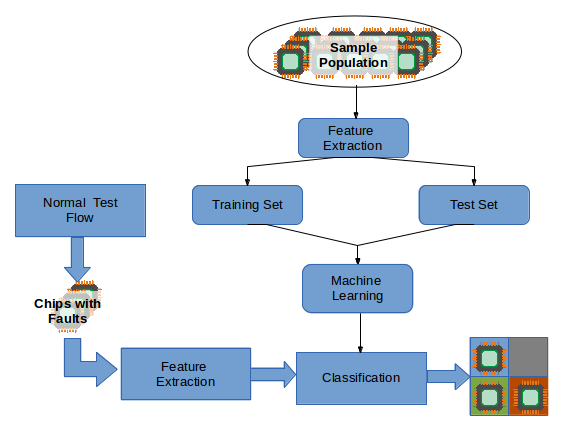
\includegraphics[scale=0.75]{figures/mlsteps.png}
    \caption{Classification of VLSI chips uning machine learning}
    \label{fig:mlsteps}
  \end{center}
\end{figure}

First step in designing a machine learning system for classification is to decide on features, which can be efficiently classify the data. Selection of proper features has the most impact in accuracy of any classifier \cite{Michie1994}. This, along with design of algorithms to extract features from input data is explained in section~\ref{sec:secfs} of this chapter. Next step is to generate sample population and decide on which machine learning algorithm is to be used, covered in next chapter.

\section{Feature Selection}
\label{sec:secfs}
To begin with feature selection, it is important to take a look at all the behavioral characteristics of different types of faults, as covered in chapter~\ref{chap:chapter2}. Table~\ref{tab:charfaults} summarizes all important characteristics to be considered for selection of features. Rest of the section describes features that were selected and algorithms for extraction of those features.

{%
\newcommand{\mc}[3]{\multicolumn{#1}{#2}{#3}}
\begin{table}[H]
 \begin{center}
  \captionsetup{justification=centering}
  \begin{tabular}{lp{4cm}p{4cm}p{4cm}}
    \mc{1}{c}{\textbf{Characteristic}} & \mc{1}{c}{\textbf{Permanent faults}} & \mc{1}{c}{\textbf{Intermittent faults}} & \mc{1}{c}{\textbf{Transient faults}}\\ \hline
    Affected outputs & Affects same set of output pins & Affects same set of output pins & Affects any of primary outputs\\
    Reproducibilty & Reproducible for same test vector & Sometimes reproducible for same test vector depending upon the error activation rate & Not preproducible\\
    Location on chip & Localized to a fault location & Localized to a fault location & Can affect any location on chip\\
    Fault behaviour & Deterministic & Deterministic & Non-deterministic \\ \hline
  \end{tabular}
  \caption{Characteristics of faults in VLSI systems}
  \label{tab:charfaults}
 \end{center}
\end{table}
}%

\subsection{Reproducibility of fault}
Reproducibility of a fault pattern during multiple test runs is defined as maximum number as maximum number of occurrence of same faulty output pattern for a fixed input pattern, and it is denoted by $\epsilon$. 

\begin{figure}[h]
  \begin{center}
    \captionsetup{justification=centering}
    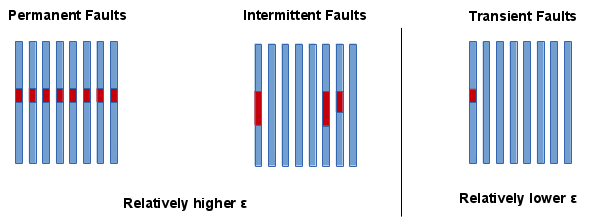
\includegraphics[scale=1.00]{figures/epsilon.png}
    \caption{Expected behavior of $\epsilon$ for different faults}
    \label{fig:epsilon}
  \end{center}
\end{figure}

Algorithm~\ref{alg:epsilon} explains extraction of $\epsilon$. It takes the expected and actual output patterns as inputs. It then checks if any of output patterns was faulty and it calculates maximum occurrences of every faulty pattern for given input pattern and stores in into array. Final value of $\epsilon$ is maximum value of in this array.

\begin{algorithm}[H]
  \caption{Algorithm to evaluate $\epsilon$}
  \label{alg:epsilon}
  \begin{algorithmic}
 \Procedure{ComputeEpsilon}{Expected output pattern array (EX), Observed output pattern array for all test runs (OP)}
 \State $\epsilon$[size(EX)] $\leftarrow$ 0\;
 \State Index $\leftarrow$ 0\;
 \While{Index $<$ size(EX)}
  \If{EX[Index] $\neq$ any pattern of OP[Index][]}
   \State $\epsilon$[Index] $\leftarrow$ max(\Call{SimilarFaultyPatterns}{OP[Index][]})\;
  \Else
   \State $\epsilon$[Index] $\leftarrow$ 0\;
  \EndIf
  \State Index++\;
 \EndWhile
 \State$\epsilon$ $\leftarrow$ max($\epsilon$[])\;
 \State \Return $\epsilon$\;
 \EndProcedure
 \end{algorithmic}
\end{algorithm}

Figure~\ref{fig:epsilon} shows expected behavior of $\epsilon$ for different fault types. Permanent faults are repeatable and value of $\epsilon$ is expected to be equal to the number of test runs for these type of faults. Intermittent faults occur at higher rate than that of transients for a fixed input pattern, hence they are also expected to have somewhat higher value than transient faults. Figure~\ref{fig:epsilonp45k} shows actual values of $\epsilon$ for a simple circuit (p45k).

\begin{figure}[h]
  \begin{center}
    \captionsetup{justification=centering}
    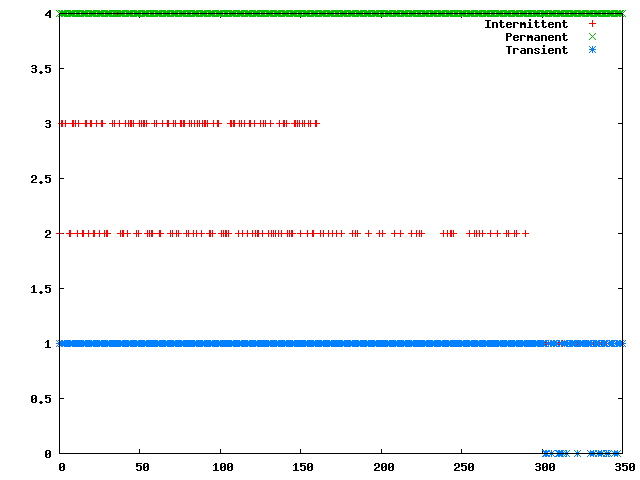
\includegraphics[scale=0.35]{figures/epsilonp45k.png}
    \caption{Plot of $\epsilon$ for p45k}
    \label{fig:epsilonp45k}
  \end{center}
\end{figure}

\subsection{Resemblance of erroneous output patterns}
Resemblance of erroneous output patterns is defined in terms of hamming distance between a set of erroneous output patterns obtained during multiple test runs, for the same input test pattern in a test set. \emph{Hamming Distance} of a set is evaluated as maximum of number of positions in which output patterns differ, pairwise. It is denoted using notation $\delta_H$, subscript $H$ stands for \enquote{horizontal}, denoting the orientation of calculation of the hamming distance. If all output patterns for an input test pattern are correct then the hamming distance and hence the value of $\delta_H$ would be zero.

\begin{figure}[h]
  \begin{center}
    \captionsetup{justification=centering}
    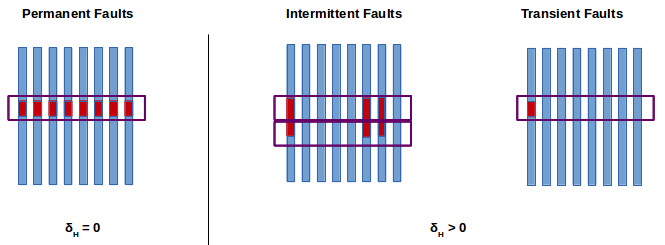
\includegraphics[scale=1.00]{figures/deltah.png}
    \caption{Expected behavior of $\delta_H$ for different faults}
    \label{fig:deltah}
  \end{center}
\end{figure}

Algorithm~\ref{alg:deltah} explains extraction of $\delta_H$. It takes the expected and actual output patterns as inputs. It then checks if any of output pattern is faulty, to save some computational efforts. If  any of output pattern is faulty, it calculates value of $\delta_H$ and stores it in array against corresponding index of input pattern. Final value of $\delta_H$ is maximum value of $\delta_H$ in this array. 

\begin{algorithm}[H]
  \caption{Algorithm to evaluate $\delta_H$}
  \label{alg:deltah}
  \begin{algorithmic}
 \Procedure{ComputeDeltaH}{Expected output pattern array (EX),Observed output pattern array for all test runs (OP)}
 \State $\delta_H$[size(EX)] $\leftarrow$ 0\;
 \State Index $\leftarrow$ 0\;
 \While{Index $<$ size(EX)}
  \If{EX[Index] $\neq$ any pattern of OP[Index][]}
   \State $\delta_H$[Index] $\leftarrow$ \Call{HammingDistance}{OP[Index][]}\;
  \Else
   \State $\delta_H$[Index] $\leftarrow$ 0\;
  \EndIf
  \State Index++\;
 \EndWhile
 \State$\delta_H$ $\leftarrow$ max($\delta_H$[])\;
 \State \Return $\delta_H$\;
 \EndProcedure
 \end{algorithmic}
\end{algorithm}

Figure~\ref{fig:deltah} shows expected behavior of $\delta_H$ for different fault types. Permanent faults repeat with same faulty output pattern and value of $\delta_H$ is expected to be zero. Intermittent faults, even though fail with same faulty output, are not repeatable and hence are expected to have a $\delta_H$ value other than zero. Transient fail randomly at random output locations and hence are expected to have higher $\delta_H$ value. Figure~\ref{fig:deltahp45k} shows actual values of $\delta_H$ for a simple circuit (p45k).

\begin{figure}[h]
  \begin{center}
    \captionsetup{justification=centering}
    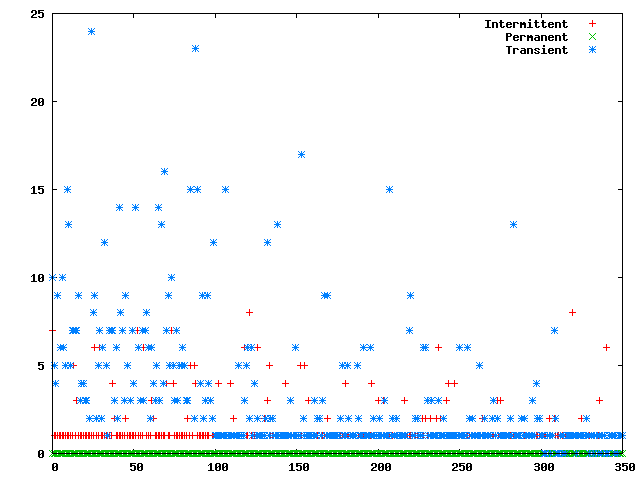
\includegraphics[scale=0.35]{figures/deltahp45k.png}
    \caption{Plot of $\delta_H$ for p45k}
    \label{fig:deltahp45k}
  \end{center}
\end{figure}

\subsection{Resemblance of erroneous primary outputs}
Resemblance of erroneous primary outputs is defined as hamming distance between primary output locations, that showed a faulty behavior at least once for a respective test run. This quantity is denoted by $\delta_V$, subscript $V$ denoting \emph{vertical} collapsing of all faulty primary outputs for a test run, before evaluating hamming distance.

Algorithm~\ref{alg:deltav} explains extraction of $\delta_V$. It takes expected output pattern and actual output patterns as inputs. It then marks the pins which showed faulty behavior at least once in a single test run of complete pattern set, as dirty. Hence number of elements in array of $\delta_V$ equals number of test runs. The final value of $\delta_V$ is hamming distance of $\delta_V$ array.

\begin{algorithm}[H]
  \caption{Algorithm to evaluate $\delta_V$}
  \label{alg:deltav}
  \begin{algorithmic}
 \Procedure{ComputeDeltaV}{Expected output pattern array (EX),Observed output pattern array for all test runs (OP)}
 \State $\delta_V$[TotalRuns] $\leftarrow$ 0\;
 \State CurrentRun $\leftarrow$ 0\;
 \While{CurrentRun $<$ TotalRuns}
  \State Index $\leftarrow$ 0\;
  \While{Index $<$ size(EX)}
	\State ExpectedOutput $\leftarrow$ EX[Index]\;
	\State ActualOutput $\leftarrow$ OP[Index][CurrentRun]\;
   \State Iterator $\leftarrow$ 0\;
	\While{Iterator $<$ length(ExpectedOutput)}
		\If{ExpectedOutput.CharAt(Iterator) $\neq$ ActualOutput.CharAt(Iterator)}
		 \State $\delta_V$[CurrentRun].CharAt(Iterator) $\leftarrow$ 1\;
		\Else
		 \State $\delta_V$[CurrentRun].CharAt(Iterator) $\leftarrow$ 0\;
		\EndIf
		\State Iterator++\;
		\EndWhile
	\State Index++\;
  \EndWhile
 \State CurrentRun++\;
 \EndWhile
 \State $\delta_V$ $\leftarrow$ \Call{HammingDistance}{$\delta_V$[]}\;
 \State \Return $\delta_V$\;
 \EndProcedure
 \end{algorithmic}
\end{algorithm}

It is expected that value of $\delta_V$ is low in case of permanent and intermittent faults, as these faults manifest into failures at fixed set of output pins. In contrast, transient faults do not have a fixed set of outputs that it affects,resulting in high expected value of $\delta_V$.  Figure~\ref{fig:deltavp45k} shows actual values of $\delta_V$ for a simple circuit (p45k).

\begin{figure}[h]
  \begin{center}
    \captionsetup{justification=centering}
    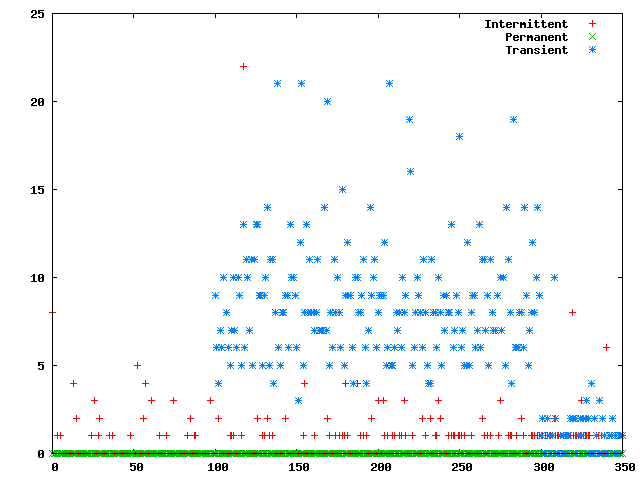
\includegraphics[scale=0.35]{figures/deltavp45k.png}
    \caption{Plot of $\delta_V$ for p45k}
    \label{fig:deltavp45k}
  \end{center}
\end{figure}

\subsection{Diagnostic features}
Diagnostic features from section~\ref{sec:secfd} are also considered as features for learning algorithm. Diagnostic data also provides information about fault present in circuit. A short summery of fault models and observed behavior for diagnostic parameters is summarized in table~\ref{tab:diagparam}. This table is taken from original work by Holst \emph{et.al.} \cite{Holst2009}.

{%
\newcommand{\mc}[3]{\multicolumn{#1}{#2}{#3}}
\begin{table}[h]
    \label{tab:diagparam}
	\captionsetup{justification=centering}
    \begin{tabular}{lccc}
	\hline
    \mc{1}{c}{\textbf{Fault Model}}        & \mc{1}{c}{\textbf{$\iota_T$}} & \mc{1}{c}{\textbf{$\tau_T$}} & \mc{1}{c}{\textbf{$\gamma_t$}} \\
	\hline
    Single stuck-at                       & 0      & 0     & 0       \\
    Stuck-at, multiple fault sites        & 0      &  > 0  & 0       \\
    Single conditional stuck-at           &  > 0   & 0     & 0       \\
    Cond. stuck-at, multiple fault sites  &  > 0   &  > 0  & 0       \\
    Delay fault, i.e. long paths fail     &  > 0   & 0     & > 0     \\ 
	\hline
    \end{tabular}
    \caption {Fault evidence compared with fault models}
\end{table}
}%

In this work it is assumed that at most only a single intermittent or permanent fault is active in the circuit with or without some transient noise (Reference to assumptions section in chap 5). Most of permanent faults can be modeled as single stuck-at, single conditional stuck-at or a delay faults. Transient faults can be modeled as conditional stuck-at faults, at multiple fault sites as the do not have a fixed location on chip and some deterministic probability function can be used as trigging condition. Similarly intermittent faults can be modeled as single conditional stuck-at faults. Hence combination of values of parameters can be used to deduce which type of fault might exist on the chip.

Furthermore, the standard deviation of evidence parameters is expected to be around zero for permanent faults, as once they are detected then they always be detected using same test pattern set. Hence as standard deviations of evidence based features convey some information about fault class, they also considered as features for learning. Figure~\ref{fig:sdevidance} shows actual values of standard deviation of evidence based features for a simple circuit (p45k).

\begin{figure}
        \centering
			\captionsetup{justification=centering}
        \begin{subfigure}[h]{0.45\linewidth}
                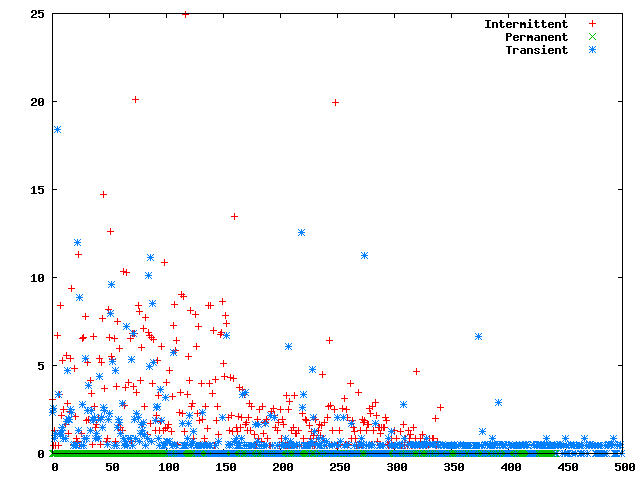
\includegraphics[scale=0.25]{figures/sdsigmap45k.png}
                \caption{Sigma ($\sigma$)}
        \end{subfigure}
        \begin{subfigure}[h]{0.45\linewidth}
                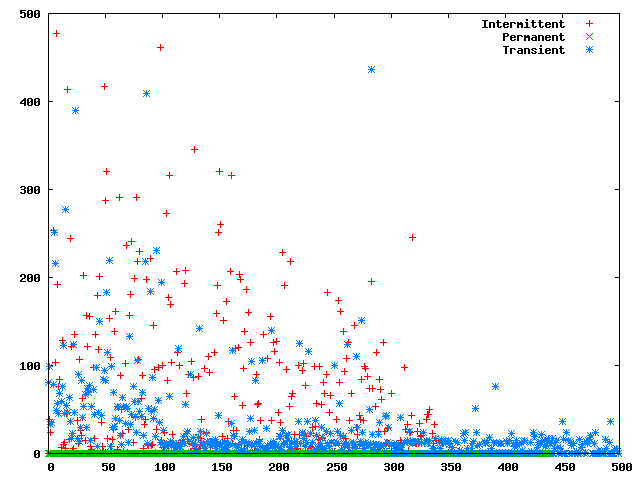
\includegraphics[scale=0.25]{figures/sdiotap45k.png}
                \caption{Iota ($\iota$)}
        \end{subfigure}
			\begin{subfigure}[h]{0.45\linewidth}
                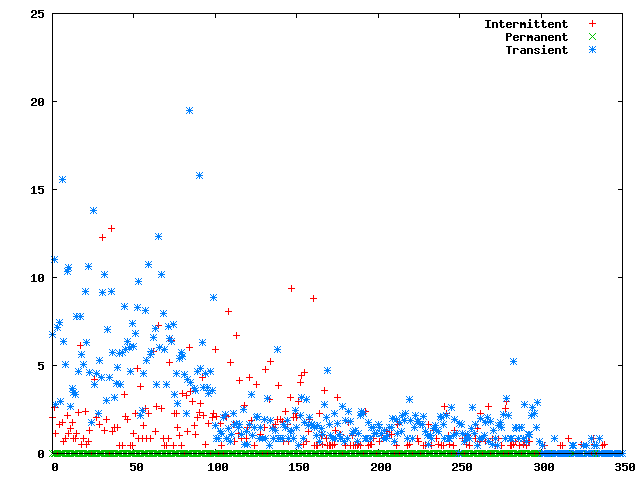
\includegraphics[scale=0.25]{figures/sdtaup45k.png}
                \caption{Tau ($\tau$)}
        \end{subfigure}
        \caption{Standard deviations for evidence-based parameters for p45k}
        \label{fig:sdevidance} 
\end{figure}

Table~\ref{tab:features} summarizes the selected features.
{%
\newcommand{\mc}[3]{\multicolumn{#1}{#2}{#3}}
\label{tab:features}
\captionsetup{justification=centering}
\begin{table}[h]
\begin{tabular}{lll}
\hline
\mc{1}{c}{\textbf{Category}}        & \mc{1}{c}{\textbf{Feature}}       & \mc{1}{c}{\textbf{Symbol}}\\
\hline
\multirow{3}{*}{Non-evidence based features} & Reproducible of fault                    & $\sigma$\\
                                             & Resemblance of erroneous output patterns  & $\delta_H$\\
                                             & Resemblance of erroneous primary outputs   & $\delta_V$\\
\hline
\multirow{8}{*}{Evidence based features}     & Maximum $\sigma$ among all test runs          & $\sigma$\\
                                             & $\iota$ corresponding to maximum $\sigma$  & $\iota$                             \\
                                             & $\tau$ corresponding to maximum $\sigma$   & $\tau$ \\
                                             & $\gamma$ corresponding to maximum $\sigma$ & $\gamma$ \\
                                             & Standard deviation of $\sigma$             & SD($\sigma$)\\
                                             & Standard deviation of $\iota$              & SD($\iota$)\\
                                             & Standard deviation of $\tau$               & SD($\tau$)\\
                                             & Standard deviation of $\gamma$             & SD($\gamma$)\\
\hline
\end{tabular}
\caption{Summary of selected features}
\end{table}
}%

\section{Selection of machine learning algorithm for fault classification}
\label{sec:selml}

There are variety of machine learning algorithms available, and some of the important ones were surveyed in chapter~\ref{chap:chapter3}. The accuracy of machine learning classifier depends mainly on the complexity of the feature space and actual training data at hand. Now that the feature set known, selection of classifier is done with respect to the following factors:

\begin{description}
  \item[Feature set] The feature set is not statistically independent, an important consideration as it violates the prerequisite for Bayes classifier. It can be seen from plots presented in section~\ref{sec:secfs}, that the feature space has high variance and it is not linearly separable, thus it is not practical to come up with rules to classify faults and hence, the performance of decision trees can be expected to be on the lower side. Also, as the feature space is highly complex, polynomial functions in MLPs might not be sufficient to create an acceptable hypothesis, can take long time to train using higher order polynomials and can result overfitting the training data. SVMs, on the other hand can handle kernel functions and can be expected to create a complex hypothesis, as required in our case.

  \item[Sample population] Size of our training data set is limited, as it needs to be generated on a simulator(refer section~\ref{sec:gsp}). Neural networks and decision trees are known to work well with large training sets \cite{DeFries2000,Tanwani2009}. On the other hand, SVMs are shown to be effective with limited size of data sets\cite{Koggalage2004}. The sample population that we have used is not created according to the probabilities of fault occurrence in real world data. It is also not possible to do so otherwise because of two main reasons, first, it is hard to get hands on actual production numbers for evaluation of results, as those numbers a closely guarded company secrets. And second, in actual application scenario, it is hard to predict probabilities of fault occurrence. This makes impossible to set set up prior probabilities required for Bayes classifier.
\end{description}

With this, it becomes clear that SVM can be used as classifier of choice as:
\begin{itemize}
  \item SVMs can work well with small and medium size data sets, with relatively high accuracy \cite{Koggalage2004, Matlab2014}.
  \item They can handle n-dimensional feature spaces.
  \item By construction, they can handle complex of feature spaces with use of kernel functions.
  \item Once trained, they are fast to classify data .
\end{itemize}